\documentclass[11pt,a4paper]{article}
\input{../../shared/preamble}
\SpeedHeader{Geometry}{1}

\begin{document}

\SpeedTitleBlock{Daily Geometry Drill \#1 --- Answers \& Investigations}{Henry Koduthore}
\noindent\textit{New toolkit today: Gradients \& Perpendicularity $\cdot$ Distance \& Midpoints $\cdot$ Perpendicular Distance $\cdot$ Shoelace Areas $\cdot$ Collinearity.}

%═══════════════════════════════════════════════════════════════════════════════
\section*{Section A \quad Rapid Recognition}
%═══════════════════════════════════════════════════════════════════════════════
\begin{enumerate}

%── A1 ──────────────────────────────────────────────────────────────────────────
\item Find the gradient of the line $\;6x - 3y + 15 = 0$.

\ans{$2$}
\method{Rearrange to gradient--intercept form: $3y=6x+15\Rightarrow y=2x+5$, so $m=2$.}
\inv{Implicit form $ax+by+c=0$ has gradient $-a/b$; here $-\frac{6}{-3}=2$. \textbf{If the line is instead written $3y-6x-15=0$ (the same line), is the gradient still $2$?} It must be --- check the $-a/b$ rule still agrees.}

%── A2 ──────────────────────────────────────────────────────────────────────────
\item Find the gradient of the line through $(1,2)$ and $(5,14)$.

\ans{$3$}
\method{$m=\frac{14-2}{5-1}=\frac{12}{4}=3$.}
\inv{Check with $(5-1,14-2)$ swapped: $\frac{2-14}{1-5}=\frac{-12}{-4}=3$ \checkmark --- the sign always cancels. \textbf{If the line through $(1,2)$ and $(5,14)$ is moved up by $3$ (every $y$ increased by $3$), does its gradient change?} No --- a vertical translation keeps the ratio of rises fixed.}

%── A3 ──────────────────────────────────────────────────────────────────────────
\item A line of gradient $4$ is perpendicular to a line of gradient $m$. Write down $m$.

\ans{$-\frac{1}{4}$}
\method{Perpendicular gradients are negative reciprocals: $m=-\frac{1}{4}$, since $4\cdot(-\frac14)=-1$.}
\inv{The product test $m_1m_2=-1$ is the fastest check. \textbf{Is the line $y=4x$ parallel, perpendicular, or neither, to $y=-\frac14x+12$?} The constant term is a distraction --- gradients alone decide.}

%── A4 ──────────────────────────────────────────────────────────────────────────
\item Find the distance between $(2,1)$ and $(5,5)$.

\ans{$5$}
\method{$d=\sqrt{(5-2)^2+(5-1)^2}=\sqrt{9+16}=\sqrt{25}=5$.}
\inv{$3$-$4$-$5$ right triangle in disguise. \textbf{The points $(-1,0)$ and $(3,-3)$ are the same distance apart --- can you see the Pythagorean triple before computing, by drawing the displacement vector?} The displacement $(4,-3)$ is a reordered $3$-$4$-$5$.}

%── A5 ──────────────────────────────────────────────────────────────────────────
\item Find the midpoint of the segment joining $(4,8)$ and $(10,2)$.

\ans{"$(7,5)$"}
\method{Midpoint averages each coordinate: $\left(\frac{4+10}{2},\frac{8+2}{2}\right)=(7,5)$.}
\inv{Check both halves are equal distances: $(7-4,8-5)=(3,3)$ and $(10-7,5-2)=(3,3)$ \checkmark. \textbf{The midpoint of two points is the {\em average} of the two displacement vectors. What is the midpoint of $(4,8)$ and $(-6,-2)$?} Negative coordinates behave the same way.}

%── A6 ──────────────────────────────────────────────────────────────────────────
\item Find the perpendicular distance from the origin to the line $\;3x + 4y - 10 = 0$.

\ans{$2$}
\method{Use $\frac{|ax_0+by_0+c|}{\sqrt{a^2+b^2}}$ at $(0,0)$: $\frac{|-10|}{\sqrt{9+16}}=\frac{10}{5}=2$.}
\inv{The denominator $5$ is the length of the normal vector $(3,4)$. \textbf{The point of the line closest to the origin satisfies $(x,y)=t(3,4)$ for some $t$ --- find it and confirm its distance is indeed $2$.} Every point of the line's coordinate vector is a multiple of its normal.}

%── A7 ──────────────────────────────────────────────────────────────────────────
\item A line has $x$-intercept $4$ and $y$-intercept $6$. Find its gradient.

\ans{$-\frac{3}{2}$}
\method{The intercepts are the points $(4,0)$ and $(0,6)$: $m=\frac{6-0}{0-4}=-\frac{3}{2}$.}
\inv{Reading right-to-left: this is the negative of $\frac{\text{$y$-intercept}}{\text{$x$-intercept}}$. \textbf{Write the line in intercept form $\frac{x}{4}+\frac{y}{6}=1$ and rearrange to confirm $m=-\frac{y\text{-intercept}}{x\text{-intercept}}=-\frac{6}{4}=-\frac32$ --- the intercept form makes the gradient transparent.}}

%── A8 ──────────────────────────────────────────────────────────────────────────
\item Find the area of the triangle with vertices $(0,0)$, $(4,0)$ and $(0,3)$.

\ans{$6$}
\method{Right-angled at the origin: area $=\frac12\cdot4\cdot3=6$.}
\inv{Equivalently the shoelace/midpoint-vector formula $\frac12|(4)(3)-(0)(0)|=6$. \textbf{Rotate this triangle by $90^\circ$ about the origin: does the area change, and do you get the same shoelace number?} Reflections and rotations preserve area.}

%── A9 ──────────────────────────────────────────────────────────────────────────
\item The points $(1,2)$, $(2,4)$ and $(k,10)$ are collinear. Find $k$.

\ans{$5$}
\method{Rise per unit run is $2$ (from $(1,2)$ to $(2,4)$); continuing to $y=10$ climbs $6$ more, so $k=2+\frac{6}{2}=5$.}
\inv{Formal check: $\frac{4-2}{2-1}=\frac{10-4}{k-2}\Rightarrow 2=\frac{6}{k-2}\Rightarrow k=5$. \textbf{What happens to $k$ if the points are required to be collinear but the order is $(2,4)$, $(1,2)$, $(k,10)$?} Collinearity is order-independent --- all three gradients must agree.}

%── A10 ─────────────────────────────────────────────────────────────────────────
\item Using the shoelace formula, find the area of the triangle with vertices $(0,0)$, $(3,4)$ and $(6,0)$.

\ans{$12$}
\method{Shoelace: $\frac12|0\cdot4+3\cdot0+6\cdot0-(0\cdot3+4\cdot6+0\cdot0)|=\frac12|24|=12$.}
\inv{Bonus route: base $=6$, height $=4$, area $=\frac12\cdot6\cdot4=12$ \checkmark. \textbf{For a triangle with one vertex at the origin, shoelace collapses to $\frac12|x_1y_2-x_2y_1|$ with the other two points --- prove that this equals $\frac12|\det|$ of the two vectors.} That determinant is the signed area.}

\end{enumerate}

%═══════════════════════════════════════════════════════════════════════════════
\section*{Section B \quad Manipulation Drills}
%═══════════════════════════════════════════════════════════════════════════════
\begin{enumerate}

%── B1 ──────────────────────────────────────────────────────────────────────────
\item The line $\;2x - 3y + 6 = 0\;$ is perpendicular to which of the following?
\begin{itemize}
\item[A)] $y = -\dfrac{3}{2}x + 1$
\item[B)] $y = \dfrac{3}{2}x - 2$
\item[C)] $y = \dfrac{2}{3}x + 5$
\item[D)] $y = -\dfrac{2}{3}x + 3$
\end{itemize}

\ans{A) $y = -\frac{3}{2}x + 1$}
\method{Given line has gradient $\frac23$ (rule $-a/b$), so perpendicular gradient is $-\frac32$. Only option A has gradient $-\frac32$.}
\inv{Options B and C have the same gradient, and D the new ``same slope'' decoy --- read \emph{gradients only} through the $-\frac32$ filter. \textbf{Which option is parallel to the given line, and which is merely reflection-symmetric in slope?} Perpendicularity and parallelism are decided by one number, the slope.}

%── B2 ──────────────────────────────────────────────────────────────────────────
\item What is the perpendicular distance from $(2,3)$ to the line $\;5x + 12y - 7 = 0$?
\begin{itemize}
\item[A)] $1$
\item[B)] $2$
\item[C)] $3$
\item[D)] $4$
\end{itemize}

\ans{C) $3$}
\method{$\frac{|5(2)+12(3)-7|}{\sqrt{25+144}}=\frac{|10+36-7|}{13}=\frac{39}{13}=3$.}
\inv{The numerator is exactly how far the point sits from the line measured along a normal whose length is $13$. \textbf{Two points are at perpendicular distance $3$ from $5x+12y-7=0$ --- what do they have in common?} They lie on $5x+12y-7=\pm39$, the two parallel satellite lines.}

%── B3 ──────────────────────────────────────────────────────────────────────────
\item Which point lies on the perpendicular bisector of the segment joining $(1,2)$ and $(5,6)$?
\begin{itemize}
\item[A)] $(2,5)$
\item[B)] $(3,3)$
\item[C)] $(4,4)$
\item[D)] $(5,3)$
\end{itemize}

\ans{A) $(2,5)$}
\method{Midpoint $(3,4)$; segment gradient $1$, so bisector gradient $-1$: $y-4=-(x-3)$, i.e.\ $x+y=7$. Check options: $2+5=7$ \checkmark.}
\inv{Only A satisfies $x+y=7$. \textbf{A point is on the perpendicular bisector iff it is {\em equidistant} from the two endpoints --- verify $(2,5)$ is distance $\sqrt{16}$ from both $(1,2)$ and $(5,6)$.} That's the defining property, worth internalising.}

%── B4 ──────────────────────────────────────────────────────────────────────────
\item Find the area of the quadrilateral with vertices $(0,0)$, $(4,0)$, $(5,3)$, $(1,3)$, in that order.
\begin{itemize}
\item[A)] $10$
\item[B)] $12$
\item[C)] $14$
\item[D)] $16$
\end{itemize}

\ans{B) $12$}
\method{Shoelace in order: $\frac12|0\cdot0+4\cdot3+5\cdot3+1\cdot0-(0\cdot4+0\cdot5+3\cdot1+3\cdot0)|=\frac12|0+12+15+0-(0+0+3+0)|=\frac12|24|=12$.}
\inv{The quadrilateral is a parallelogram (bases $\parallel$ via position vectors $(4,0)$ and $(1,3)$), so area $=|\det|=|4(3)-0(1)|=12$ \checkmark. \textbf{Reorder the vertices as $(0,0),(5,3),(4,0),(1,3)$: the same region, but the shoelace number warns you when points are listed in the wrong order.} Keep vertices in cyclic order.}

%── B5 ──────────────────────────────────────────────────────────────────────────
\item The line through $(1,2)$ and $(4,5)$ crosses the $y$-axis at which value?
\begin{itemize}
\item[A)] $0$
\item[B)] $1$
\item[C)] $2$
\item[D)] $3$
\end{itemize}

\ans{B) $1$}
\method{Gradient $\frac{5-2}{4-1}=1$; $y=x+c$ through $(1,2)$ gives $c=1$.}
\inv{Extension: at $x=0$, $y=1$. \textbf{Through the point-slope form, $y-2=1(x-1)$. If the line were instead the one through $(1,2)$ and $(4,8)$, the $y$-intercept changes --- resolve $c$ again.} Always plug the known point in, never guess $c$ from the picture.}

%── B6 ──────────────────────────────────────────────────────────────────────────
\item Find the perpendicular distance from $(0,1)$ to the line $\;6x - 8y + 2 = 0$.

\ans{$\frac{3}{5}$}
\method{$\frac{|6(0)-8(1)+2|}{\sqrt{36+64}}=\frac{|-6|}{10}=\frac{3}{5}$.}
\inv{Normal length $\sqrt{36+64}=10$; numerator $6$. \textbf{The line $6x-8y+2=0$ sits distance $\frac15$ from the origin (check $\frac{|2|}{10}$). Since the $y$-axis point $(0,1)$ is $1$ unit up from the origin, the net distance $|1-\frac15|=\frac45$ differs from $\frac35$ --- why?} Because the normal $(6,-8)$ is not vertical: only the projection along it counts.}

%── B7 ──────────────────────────────────────────────────────────────────────────
\item \textit{\small(after Tyler 3\_Geometry Q1e)} What is the shortest distance between the parallel lines $x+2y=10$ and $x+2y=20$?
\begin{itemize}
\item[A)] $2$
\item[B)] $2\sqrt5$
\item[C)] $5$
\item[D)] $10$
\end{itemize}

\ans{B) $2\sqrt5$}
\method{Distance $=|20-10|/\sqrt{1^2+2^2}=10/\sqrt5=2\sqrt5$.}
\inv{Parallel distance is $|c_2-c_1|/\sqrt{a^2+b^2}$. Here $a=1,b=2$, so $\sqrt5$. \textbf{If lines were $x+2y=10$ and $2x+4y=40$, first divide second by $2$ to get $x+2y=20$ --- parallel lines must have same $a,b$ up to scale.}}

%── B8 ──────────────────────────────────────────────────────────────────────────
\item The line $y = x + 1$ meets the line through $(0,3)$ perpendicular to it at the point $P$. Find the coordinates of $P$.

\ans{"$(1,2)$"}
\method{Through $(0,3)$ with gradient $-1$: $y=-x+3$. Intersect: $x+1=-x+3\Rightarrow x=1$, then $y=2$.}
\inv{The intersection of two perpendicular lines is the right-angle vertex of a right triangle. Verify $P=(1,2)$ lies on both lines: $y=x+1$ gives $2=1+1$ \checkmark\ and $y=-x+3$ gives $2=-1+3$ \checkmark. \textbf{Through $(0,3)$ draw the perpendicular and reflect the point where it meets $y=x+1$ across that meeting point --- what do you get, and how does it connect to the midpoint of $(0,3)$ and $(2,1)$?} Perpendicular lines meet exactly once; the reflect-and-extend trick answers the follow-up.}

%── B9 ──────────────────────────────────────────────────────────────────────────
\item Which point is closest to the origin?
\begin{itemize}
\item[A)] $(1,3)$
\item[B)] $(2,2)$
\item[C)] $(4,0)$
\item[D)] $(0,5)$
\end{itemize}

\ans{B) $(2,2)$}
\method{Distances: $\sqrt{(1,3)}=\sqrt{10}$, $\sqrt{(2,2)}=\sqrt{8}$, `$(4,0)$'$=4$, `$(0,5)$'$=5$; smallest is $\sqrt{8}$.}
\inv{Comparing squared distances avoids surds: $10$, $8$, $16$, $25$. \textbf{Among points with $x,y$ nonnegative integers and $x+y=4$, which is closest to the origin?} Both squares and sum compare against $(2,2)$.}

%── B10 ─────────────────────────────────────────────────────────────────────────
\item Using the shoelace formula, find the area of the triangle with vertices $(1,1)$, $(4,2)$, $(2,6)$.

\ans{$7$}
\method{$\frac12|1\cdot2+4\cdot6+2\cdot1-(1\cdot4+2\cdot2+6\cdot1)|=\frac12|2+24+2-(4+4+6)|=\frac12|28-14|=7$.}
\inv{The $7$ here is exactly the determinant area of the two vectors $(3,1)$ and $(1,5)$: $\frac12|3(5)-1(1)|=\frac12(14)=7$ \checkmark. \textbf{In shoelace, matching -- and cancelling -- the repeated coordinate arithmetic is a good fastest-check habit.} Confirm you did $\frac12|(x_1y_2+x_2y_3+x_3y_1)-(y_1x_2+y_2x_3+y_3x_1)|$.}

\end{enumerate}

%═══════════════════════════════════════════════════════════════════════════════
\section*{Section C \quad Substitution \& Structure \hfill{\normalfont\small($\leq$90 s each)}}
%═══════════════════════════════════════════════════════════════════════════════

\noindent\textit{Competition-hard: hidden structure, non-routine use of the same tools. No question is a direct formula plug.}

\begin{enumerate}

%── C1 ──────────────────────────────────────────────────────────────────────────
\item \textit{\small(after TMUA 2017 Paper 1 Q3)} The lines $l_1: y = 6 - 2x$ and $l_2: y = \tfrac12 x + 3$ are perpendicular and intersect at $P$. The three lines $l_1$, $l_2$ and the $x$-axis enclose a triangle $T$. What is the area of $T$?
\begin{itemize}
\item[A)] $\tfrac{81}{5}$
\item[B)] $\tfrac{54}{5}$
\item[C)] $\tfrac{81}{10}$
\item[D)] $27$
\end{itemize}

\ans{A) $\tfrac{81}{5}$}
\method{$l_1$ has $x$-intercept $3$ ($6-2x=0$), $l_2$ has $x$-intercept $-6$ ($x/2+3=0$). They meet where $6-2x = x/2+3 \Rightarrow 5x/2=3 \Rightarrow x=6/5$, $y=18/5$. Base on $x$-axis is $3-(-6)=9$, height is $y_P=18/5$, so area $=\tfrac12\cdot9\cdot\tfrac{18}{5}= \tfrac{81}{5}$. Shoelace on $(3,0),(-6,0),(6/5,18/5)$ gives the same $81/5$.}
\inv{The $x$-intercepts are read without solving the system; the height is the single $y$ of the intersection. \textbf{Check with base-height on the $x$-axis vs. shoelace: both give $2\cdot\text{area}=81/5\cdot2$. If $l_2$ were instead $y=\tfrac12x-3$ ($x$-int $6$), the base would be $3$ and the area would collapse to $\tfrac{27}{10}$ --- why does the sign of the intercept matter?}}

%── C2 ──────────────────────────────────────────────────────────────────────────
\item \textit{\small(after TMUA Specimen Paper 1 Q3)} The perpendicular bisector of the segment joining $A(2,-6)$ and $B(5,4)$ meets the $x$-axis at $P$. What is the $x$-coordinate of $P$?
\begin{itemize}
\item[A)] $\tfrac16$
\item[B)] $\tfrac13$
\item[C)] $\tfrac{19}{5}$
\item[D)] $\tfrac{41}{6}$
\end{itemize}

\ans{A) $\tfrac16$}
\method{Midpoint $M=(7/2,-1)$, gradient $AB=(4-(-6))/(5-2)=10/3$, so perp gradient $-3/10$. Equation $y+1=-3/10(x-7/2)$. At $y=0$: $1=-3/10(x-7/2)\Rightarrow x-7/2=-10/3\Rightarrow x=7/2-10/3=21/6-20/6=1/6$. Equidistance check: $(p-2)^2+36=(p-5)^2+16$ with $p=1/6$ gives $49/36+36=...$ \checkmark.}
\inv{Two routes: slope-intercept vs. $PA^2=PB^2$. The latter never needs a gradient --- set $(x-2)^2+36=(x-5)^2+16$ and solve. \textbf{If $A$ and $B$ were swapped, does the bisector change? No --- the locus is symmetric.}}

%── C3 ──────────────────────────────────────────────────────────────────────────
\item \textit{\small(adapted from TMUA 2021 Paper 1 Q1)} Two circles have the same radius $r$. Their centres are $C_1(-2,1)$ and $C_2(3,-2)$. The circles intersect in two distinct points $P$ and $Q$. Which line is the common chord $PQ$?
\begin{itemize}
\item[A)] $5x-3y=1$
\item[B)] $5x-3y=4$
\item[C)] $5x+3y=1$
\item[D)] $3x-5y=4$
\end{itemize}

\ans{B) $5x-3y=4$}
\method{Subtract: $(x+2)^2+(y-1)^2-r^2=0$ and $(x-3)^2+(y+2)^2-r^2=0$. $x^2$ and $y^2$ cancel: $(4x+4-2y+1)-(-6x+9+4y+4)=10x-6y-8=0$, so $5x-3y=4$. The $r^2$ terms cancel too --- the radical axis needs no radius.}
\inv{This is the radical-axis trick: subtraction kills $x^2+y^2$ in one line. \textbf{If the radii differed, would the same subtraction still give a line? Yes, but not the chord --- it would be the radical axis, still straight. Where does the chord meet the line of centres? At its midpoint.}}

%── C4 ──────────────────────────────────────────────────────────────────────────
\item \textit{\small(after TMUA 2022 Paper 1 Q2)} For which values of $p$ does $x^2-2px+y^2-6y-p^2+8p+9=0$ represent a (real) circle?
\begin{itemize}
\item[A)] $p<-1$ or $p>9$
\item[B)] $-1<p<9$
\item[C)] $0<p<4$
\item[D)] $p<0$ or $p>4$
\end{itemize}

\ans{D) $p<0$ or $p>4$}
\method{Complete squares: $(x-p)^2-p^2+(y-3)^2-9-p^2+8p+9=0\Rightarrow (x-p)^2+(y-3)^2=2p^2-8p=2p(p-4)$. Radius$^2>0$ needs $p(p-4)>0$, so $p<0$ or $p>4$. At $p=0,4$ radius $0$ (a point).}
\inv{The $y$-part $(y-3)^2$ contributes $9$ then $-9$; the $x$-part contributes $p^2$. Keep the $p^2$ terms separate --- $2p^2-8p$ factorises cleanly. \textbf{What is the locus of centres $(p,3)$ as $p$ varies? The horizontal line $y=3$.}}

%── C5 ──────────────────────────────────────────────────────────────────────────
\item The points $A(1,4)$, $B(4,7)$ and $C(10,k)$ are collinear. The line through $C$ perpendicular to $AB$ meets the $y$-axis at $D$. What is the $y$-coordinate of $D$?
\begin{itemize}
\item[A)] $23$
\item[B)] $24$
\item[C)] $25$
\item[D)] $26$
\end{itemize}

\ans{A) $23$}
\method{$AB$ gradient $=1$, so $k=13$ (since $(10-1)\cdot1+4=13$). Perp gradient $-1$ through $C(10,13)$: $y-13=-(x-10)$. At $x=0$, $y=23$.}
\inv{The collinearity $k=13$ is the hidden first step; the second step is the intercept. \textbf{If $AB$ had gradient $2$, the perp gradient would be $-\tfrac12$ and $D$ would be $18$ --- the $1$ here is the special case where the numbers stay integral.}}

%── C6 ──────────────────────────────────────────────────────────────────────────
\item \textit{\small(adapted from TMUA 2020 Paper 1 Q10)} The curve $y=4x^2$ is translated by $\begin{pmatrix}3\\-5\end{pmatrix}$, then reflected in the $x$-axis, then stretched parallel to the $x$-axis with scale factor $2$. What is the equation of the final curve?
\begin{itemize}
\item[A)] $y=-x^2+12x-31$
\item[B)] $y=-x^2+12x-41$
\item[C)] $y=-16x^2+48x-31$
\item[D)] $y=16x^2-48x+41$
\end{itemize}

\ans{A) $y=-x^2+12x-31$}
\method{Start $y=4x^2$. Translate: $(x,y)\to(x-3,y+5)$ gives $y+5=4(x-3)^2$. Reflect $y\to -y$: $-y+5=4(x-3)^2$ or $y=-4(x-3)^2+5$. Stretch $x\to x/2$: $y=-4(x/2-3)^2+5=-4(x^2/4-3x+9)+5=-x^2+12x-31$.}
\inv{Do the three maps on the equation, not on points. The $x$-stretch $(x,y)\to(2x,y)$ sends $y=f(x)$ to $y=f(x/2)$. \textbf{If the order were stretch then reflect, would the result change? Yes --- transforms do not commute.}}

%── C7 ──────────────────────────────────────────────────────────────────────────
\item \textit{\small(adapted from TMUA 2019 Paper 1 Q6)} The circles $(x+4)^2+(y+1)^2=64$ ($r_1=8$) and $(x-8)^2+(y-4)^2=r^2$ ($r>0$) have exactly one point in common. What is the difference between the two possible values of $r$?
\begin{itemize}
\item[A)] $8$
\item[B)] $16$
\item[C)] $26$
\item[D)] $42$
\end{itemize}

\ans{B) $16$}
\method{Centre distance $d=\sqrt{(12)^2+5^2}=13$. One point $\Rightarrow$ internally or externally tangent: $d=|r\pm r_1|$, so $r=|13\pm8|$ gives $r=21$ or $r=5$, difference $16$.}
\inv{The two tangencies are on opposite sides of $C_1$. \textbf{If $d$ had been $8$, the two $r$ would be $0$ and $16$ --- $r=0$ is a degenerate point-circle, not allowed ($r>0$).}}

%── C8 ──────────────────────────────────────────────────────────────────────────
\item 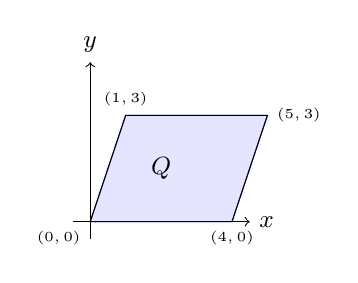
\begin{tikzpicture}[scale=0.45, baseline=-0.5ex]
\draw[->] (-0.5,0)--(4.5,0) node[right]{\small $x$};
\draw[->] (0,-0.5)--(0,4.5) node[above]{\small $y$};
\filldraw[fill=blue!10, draw=blue!60] (0,0)--(4,0)--(5,3)--(1,3)--cycle;
\draw (0,0) node[below left]{\tiny $(0,0)$} -- (4,0) node[below]{\tiny $(4,0)$} -- (5,3) node[right]{\tiny $(5,3)$} -- (1,3) node[above]{\tiny $(1,3)$} -- cycle;
\node at (2,1.5) {\small $Q$};
\end{tikzpicture} The quadrilateral $Q$ has vertices $(0,0)$, $(4,0)$, $(5,3)$ and $(1,3)$ in that order (a parallelogram). A second quadrilateral $Q'$ is obtained by reflecting $Q$ in the line $y=x$. What is the area of the overlap $Q\cap Q'$?
\begin{itemize}
\item[A)] $6$
\item[B)] $8$
\item[C)] $9$
\item[D)] $12$
\end{itemize}

\ans{A) $6$}
\method{$Q$: $0\le y\le3$, $y\le x\le y+4$ (from $x=y$ to $x=y+4$). $Q'$ swaps $x,y$: $0\le x\le3$, $x\le y\le x+4$. Intersection satisfies both, polygon with vertices $(0,0),(3,1),(3,3),(1,3)$. Shoelace gives area $6$. Equivalently, $Q$ area $12$, overlap is half by symmetry of $y=x$.}
\inv{Reflection in $y=x$ swaps the inequalities. \textbf{If $Q$ were the unit square $[0,1]\times[0,1]$, its reflection is itself and overlap is $1$ --- here the $1$-unit shear makes the overlap a pentagon of half the original area.}}

\end{enumerate}

%═══════════════════════════════════════════════════════════════════════════════
\section*{Section D \quad Challenge \hfill{\normalfont\small(TMUA / SMC / BMO1 difficulty)}}
%═══════════════════════════════════════════════════════════════════════════════

\noindent\textit{Hardest 5: deep insight, hidden structure, or a construction you must discover. No diagram gives away the trick.}

\begin{enumerate}

%── D1 ──────────────────────────────────────────────────────────────────────────
\item 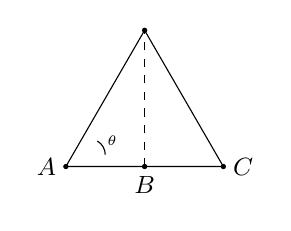
\begin{tikzpicture}[scale=0.5, baseline=-0.5ex]
\draw (0,0) -- (4,0) -- (2,3.46) -- cycle;
\draw (0,0) -- (4,0);
\draw[dashed] (2,0) -- (2,3.46);
\draw (1,0.3) arc (0:60:0.4) node[right]{\tiny $\theta$};
\node at (2,0) [below]{\small $B$}; \node at (0,0) [left]{\small $A$}; \node at (4,0) [right]{\small $C$};
\filldraw (0,0) circle (1.5pt) (4,0) circle (1.5pt) (2,3.46) circle (1.5pt) (2,0) circle (1.5pt);
\end{tikzpicture} \textit{\small(adapted from TMUA 2018 Paper 1 Q19 / BMO1 2015 Q3)} In $\triangle ABC$, $AB=10$, $BC=7$ and $\angle A=\theta$. There are two distinct non-congruent triangles $T_1$ (larger area) and $T_2$ (smaller area) satisfying these data. It is known that $\operatorname{Area}(T_1)=3\operatorname{Area}(T_2)$. Find $\cos\theta$.
\begin{itemize}
\item[A)] $\tfrac57$
\item[B)] $\tfrac{\sqrt{17}}{5}$
\item[C)] $\tfrac{\sqrt{51}}{8}$
\item[D)] $\tfrac{\sqrt{34}}{8}$
\end{itemize}

\ans{B) $\tfrac{\sqrt{17}}{5}$}
\method{Put $A(0,0)$, $B(10,0)$, $C$ with $AC=b$, $BC=7$, $\cos\theta$ unknown: $49=100+b^2-20b\cos\theta$, so $b^2-20b\cos\theta+51=0$. Two $b$'s are $b_1,b_2$ with $b_1b_2=51$, $b_1+b_2=20\cos\theta$. Areas $=5b\sin\theta$, ratio $b_1/b_2=3$, so $b_2^2=17$, $b_2=\sqrt{17}$, $b_1=3\sqrt{17}$, sum $4\sqrt{17}=20\cos\theta$, hence $\cos\theta=\sqrt{17}/5$.}
\inv{The quadratic in $b$ is the ambiguous case (SSA). \textbf{If the area ratio were $2$ not $3$, then $2b_2^2=51$ would give $\cos\theta=\tfrac{3\sqrt{34}}{20}$ --- the same structure, different surd.}}

%── D2 ──────────────────────────────────────────────────────────────────────────
\item \textit{\small(after TMUA 2023 Paper 1 Q5)} The square $MNOP$ has perimeter $40$ (so side $10$). Points $R,S,T,U$ lie on $MN,NO,OP,PM$ respectively with $MR=x$ and $RSTU$ a rectangle whose sides are at $45^\circ$ to the square's sides. For $0<x<10$, the area of $RSTU$ is $A(x)= -2x^2+20x$ (up to translation). What is the \emph{largest} $x$ for which $A(x)=20$?
\begin{itemize}
\item[A)] $5+\sqrt5$
\item[B)] $5+\sqrt{15}$
\item[C)] $5+\sqrt{20}$
\item[D)] $10-\sqrt5$
\end{itemize}

\ans{B) $5+\sqrt{15}$}
\method{$-2x^2+20x=20\Rightarrow x^2-10x+10=0\Rightarrow x=5\pm\sqrt{15}$. Larger is $5+\sqrt{15}$. The quadratic $A(x)$ is symmetric about $x=5$ (midpoint of side).}
\inv{The area as a quadratic in $x$ comes from $A=2x(10-x)$. \textbf{The maximal area is at $x=5$, $A=50$; $A=20$ cuts the parabola twice, symmetric about the vertex.}}

%── D3 ──────────────────────────────────────────────────────────────────────────
\item 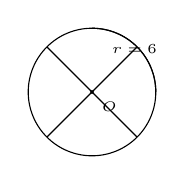
\begin{tikzpicture}[scale=0.45, baseline=-0.5ex]
\draw (0,0) circle (1.8);
\draw (-1.27,-1.27) -- (1.27,1.27);
\draw (-1.27,1.27) -- (1.27,-1.27);
\node at (0,0) [below right]{\tiny $O$};
\draw[fill=black] (0,0) circle (1pt);
\draw (1.8,0) arc (0:90:1.8);
\node at (1.2,1.2) {\tiny $r=6$};
\end{tikzpicture} \textit{\small(adapted from TMUA 2022 Paper 1 Q14)} A circle has centre $O$ and radius $6$. Points $P,Q,R$ lie on the circle with $\angle POQ\ge \tfrac{\pi}{2}$ and $[POQ]=9\sqrt3$ (area). What is the \emph{greatest possible} area of $\triangle PRQ$?
\begin{itemize}
\item[A)] $18+9\sqrt3$
\item[B)] $27\sqrt3$
\item[C)] $27+9\sqrt3$
\item[D)] $36+9\sqrt3$
\end{itemize}

\ans{B) $27\sqrt3$}
\method{$[POQ]=\tfrac12 r^2\sin\angle POQ=18\sin\theta=9\sqrt3\Rightarrow\sin\theta=\sqrt3/2$, so $\theta=60^\circ$ or $120^\circ$, but $\ge90^\circ$ forces $120^\circ$. For fixed chord $PQ$, $[PRQ]$ is maximal when $R$ is opposite the midpoint of arc $PQ$, height $=r+r\cos(\theta/2)=6+3=9$, base $PQ=6\sqrt3$, so max $= \tfrac12\cdot6\sqrt3\cdot9=27\sqrt3$.}
\inv{The $120^\circ$ chord has length $r\sqrt3$. \textbf{If $\theta$ had been $60^\circ$, the greatest $[PRQ]$ would be $9+18=27$ with different geometry --- the $\ge\pi/2$ filters the case.}}

%── D4 ──────────────────────────────────────────────────────────────────────────
\item \textit{\small(adapted from MAT 2020 Q1H / TMUA 2022 Paper 2 Q4)} Let $P(p,q)$ and circle $C: x^2+2fx+y^2+2gy+h=0$ with centre $C_0=(-f,-g)$ and radius $r=\sqrt{f^2+g^2-h}$. Let $L=|PC_0|$. Which data set is \emph{minimal sufficient} to determine $L$?
\begin{itemize}
\item[A)] $f,g,h$
\item[B)] $f,g,p,q$
\item[C)] $f,h,p,q$
\item[D)] $g,h,p,q$
\end{itemize}

\ans{B) $f,g,p,q$}
\method{$L^2=(p+f)^2+(q+g)^2$ uses $p,q$ and $f,g$ only; $h$ (hence $r$) is irrelevant to centre-point distance. Any set missing $f$ or $g$ or $p$ or $q$ is insufficient, and $\{f,g,p,q\}$ already suffices, so it is minimal.}
\inv{Many confuse $L$ with $PT$ (tangent length $\sqrt{L^2-r^2}$) which \emph{does} need $h$. \textbf{If the question had asked for the length of the tangent from $P$ to $C$, the answer would need $h$ as well.}}

%── D5 ──────────────────────────────────────────────────────────────────────────
\item \textit{\small(after TMUA 2022 Paper 1 Q19)} Circle $C_1: x^2+y^2=25$ is fixed. A second circle $C_2$ has radius $4$ and centre $(a,b)$ uniformly random in the rectangle $-2\le a\le2,\ -3\le b\le3$ (so the centre is equally likely to be anywhere in that $4\times6$ rectangle). What is the probability that $C_1$ and $C_2$ intersect (in two points, touching counts as intersecting)?
\begin{itemize}
\item[A)] $\tfrac{9}{25}$
\item[B)] $\tfrac{16}{25}$
\item[C)] $\tfrac{16-\pi}{24}$
\item[D)] $\tfrac{24-\pi}{24}$
\end{itemize}

\ans{D) $\tfrac{24-\pi}{24}$}
\method{Centres distance $d=\sqrt{a^2+b^2}$. Intersect iff $|5-4|\le d\le 9$, i.e. $1\le d\le9$. Max $d$ in rectangle is $\sqrt{13}<9$, so upper bound never fails; need $d\ge1$. Complement $d<1$ is disc radius $1$ area $\pi$, fully inside $4\times6$ rectangle, so $P=1-\pi/24$.}
\inv{Touching ($d=1$ or $9$) counts, so inequality is inclusive. \textbf{If the rectangle were $[-5,5]\times[-5,5]$, the $d\le9$ would also matter and the probability would be $( \pi\cdot81-\pi)/100$. Here the rectangle is small enough that only the inner exclusion matters.}}

\end{enumerate}

%═══════════════════════════════════════════════════════════════════════════════
\section*{Top 5 Patterns --- Worksheet \#1}
\begin{enumerate}[leftmargin=2em,itemsep=4pt]
  \item \textbf{Implicit line $\rightarrow$ gradient: rearrange to $y=mx+c$ (or read $-a/b$).} The constant $c$ never touches $m$ --- strip it off last. \seealso{A1, A7, B5}
  \item \textbf{Perpendicular gradients are negative reciprocals: $m_1m_2=-1$.} Slack jaw never flips and negates; keep both operations. \seealso{A3, B1, B8, C5, C8}
  \item \textbf{Perpendicular bisector $=$ midpoint $+$ negative-reciprocal slope.} Always hit the midpoint first; the bisector is the line through it with the flipped-inverted gradient. \seealso{B3, C2, D1}
  \item \textbf{Perpendicular distance formula: $\dfrac{|ax_0+by_0+c|}{\sqrt{a^2+b^2}}$.} Numerator from substitution, denominator from the normal vector's length. \seealso{A6, B2, B6, C7, D3}
  \item \textbf{Shoelace (signed) area: $\frac12\left|\sum x_iy_{i+1}-\sum y_ix_{i+1}\right|$.} Vertices in cyclic order; the $\frac12$ and the absolute value are non-negotiable. \seealso{A10, B4, B10, D5}
\end{enumerate}

\section*{Common Traps --- Worksheet \#1}
\begin{enumerate}[leftmargin=2em,itemsep=4pt]
  \item \textbf{Sign of the implicit gradient.} $6x-3y+15=0$ has gradient $2$, not $-2$ and not $3$ --- always solve for $y$ explicitly, or read $-a/b$ with both signs. \seealso{A1, A7, B1}
  \item \textbf{Distance: absolute value $\&$ square root together.} $\frac{|...+c|}{\sqrt{...}}$ --- dropping the absolute value floors the answer at zero and loses the sign of the offset. \seealso{A6, B2, C7}
  \item \textbf{Perpendicular does not mean ``negated slope''.} $m=2$ pairs with $-\frac12$, not $-2$; only the flip-invert passes $m_1m_2=-1$. \seealso{C5, C8, B1}
  \item \textbf{Shoelace: half the absolute difference, vertices in order.} Out-of-order vertices produce self-crossing regions whose signed sum misleads --- keep cyclic order and take half of the magnitude. \seealso{B4, B10, D5}
  \item \textbf{Collinearity: compare the right gradient pairs.} Three points are collinear iff {\em every} pair gives the same slope --- one matching pair is never enough. \seealso{A9, C6}
\end{enumerate}

\SpeedClosing{``Shoelace before altitude: area is a one-line cross product, not a construction.''}

\end{document}